\begin{tikzpicture}
    \node {a} [sibling distance = 2.0cm]
    child [] {node {
            \only<1-2>{b}\only<3->{\textcolor{blue}{b}}
            } [sibling distance =2.15cm]
        % c=1
        child [] {node {\only<3->{c}} [sibling distance = 1.35cm]
            child [] {node {x} 
                child [] {node  {\red{X}} edge from parent [] node [left]{1}}
                child [] {node {\red{X}} edge from parent [] node [right]{0}}
            edge from parent [] node [left]{0}} 
        edge from parent [] node [left]{\only<3->{1}}}
        % c=0
        child [] {node {c} [sibling distance =1.35cm]
            child [] {node {x} 
            child [] {node {\red{X}} edge from parent [] node [left]{1}}
            child [] {node {\red{X}} edge from parent [] node [right]{0}}
        edge from parent [] node [left]{0}} 
        edge from parent [] node [right]{0}}
    edge from parent [] node [left]{\only<1-2>{1}\only<3->{\textcolor{blue}{1}}}}
    child [] {node {b} 
    edge from parent [] node [right]{0}};
\end{tikzpicture}